\documentclass[compress]{beamer}

\usetheme{Hamburg}

\usepackage[T1]{fontenc}
\usepackage[utf8]{inputenc}

\usepackage{lmodern}

%\usepackage[english]{babel}
\usepackage[ngerman]{babel}

\usepackage{eurosym}
\usepackage{listings}
\usepackage{microtype}
\usepackage{units}

\makeatletter
\newcommand*{\rom}[1]{\expandafter\@slowromancap\romannumeral #1@}
\makeatother

\lstset{
	basicstyle=\ttfamily\footnotesize,
	frame=single,
	numbers=left,
	language=C,
	breaklines=true,
	breakatwhitespace=true,
	postbreak=\hbox{$\hookrightarrow$ },
	showstringspaces=false,
	tabsize=4,
	captionpos=b,
	morekeywords={gboolean,gpointer,gconstpointer,gchar,guchar,gint,guint,gshort,gushort,glong,gulong,gint8,guint8,gint16,guint16,gint32,guint32,gint64,guint64,gfloat,gdouble,gsize,gssize,goffset,gintptr,guintptr,int8_t,uint8_t,int16_t,uint16_t,int32_t,uint32_t,int64_t,uint64_t,size_t,ssize_t,off_t,intptr_t,uintptr_t,mode_t}
}

\title{SCIL - Scientific Compression Interface Library}
\author{Armin Schaare}
\institute{Arbeitsbereich Wissenschaftliches Rechnen\\Fachbereich Informatik\\Fakultät für Mathematik, Informatik und Naturwissenschaften\\Universität Hamburg}
\date{2016-01-17}

\titlegraphic{
\includegraphics[width=0.75\textwidth]{logo}}

\begin{document}

\begin{frame}
	\titlepage
\end{frame}

\begin{frame}
	\frametitle{Outline}

	\tableofcontents[hidesubsections]
\end{frame}

\section{Introduction}
\subsection*{}

\begin{frame}
	\frametitle{Scientific Compression Interface Library}

	\begin{itemize}
		\item C-Library for lossy compression
		\item User provides required precision
		\begin{itemize}
			\item Many metrics possible, currently:
			\item Relative error tolerance
			\item Absolute error tolerance
			\item Significant digits
		\end{itemize}
		\item SCIL chooses which algorithm is best suited
		\item User can force specific compression algorithms
		\begin{itemize}
			\item Useful for testing
		\end{itemize}
	\end{itemize}

\end{frame}

\begin{frame}
	\frametitle{Usage}

	\begin{itemize}
		\item Define required precision in 'scil\_hints' struct
		\item Create compression context
		\item Allocate destination buffer
		\item Use context to compress the given buffer
	\end{itemize}

\end{frame}

\begin{frame}[fragile]
	\frametitle{Usage Example Code}

	\begin{lstlisting}[caption=SCIL usage example]
	scil_hints hints;
	hints.force_compression_method = 0; //memcpy

	scil_context * ctx;
	scil_create_compression_context(&ctx, &hints);

	size_t c_size;
	scil_compress(ctx, c_buf, &c_size, u_buf, u_size);
	\end{lstlisting}

	\footnotesize{
	\begin{tabular}{ll}
		c\_buf: & allocated destination buffer \\
		c\_size: & will be byte size of c\_buf \\
		u\_buf: & uncompressed source buffer \\
		u\_size: & byte size of u\_buf
	\end{tabular}
	}

\end{frame}

\section{Approach}
\subsection{Compression}

\begin{frame}
	\frametitle{Algorithm Specific Buffer Setup}

	\begin{itemize}
		\item Use scil\_hints for algorithm choice
		\item Set up header depending on algorithm used
		\begin{itemize}
			\item Header contains relevant data for decompression
		\end{itemize}
		\item Write compressed data into rest of buffer
	\end{itemize}

	\bigskip

	General buffer setup:\\
	\begin{center}
	\begin{tabular}{|c|c|cc|}
		\hline
		id & compression info & compressed data & ... \\
		\hline
		\multicolumn{2}{|c|}{} & \multicolumn{2}{c|}{} \\
		\multicolumn{2}{c}{header} & \multicolumn{2}{c}{body}
	\end{tabular}
	\end{center}
\end{frame}

\begin{frame}
	\frametitle{Buffer Setup Examples}

	Trivial compression with memcpy:\\
	\begin{center}
	\begin{tabular}{|c||cc|}
		\hline
		0 & compressed data & ... \\
		\hline
	\end{tabular}
	\end{center}

	\bigskip
	\pause

	Using algorithm from last presentation:\\
	\begin{itemize}
		\item Compressing temperature data
		\item Smallest value: -100
		\item Error tolerance: 0.005 (hundredth degree precision)
	\end{itemize}
	\begin{center}
	\begin{tabular}{|c|c|cc|}
		\hline
		1 & -100 0.005 & compressed data & ... \\
		\hline
	\end{tabular}
	\end{center}

\end{frame}

\subsection{Decompression}

\begin{frame}
	\frametitle{Decompression Procedure}

	\begin{itemize}
		\item Read in compressed buffer
		\item Decide which algorithm to use from first byte (algo-id)
		\item Use comp. information as parameters in decomp. function
		\item Decompress the data

	\end{itemize}
\end{frame}

\section{Conclusion}
\subsection*{}

\begin{frame}
	\frametitle{Benchmark}
	\begin{center}
		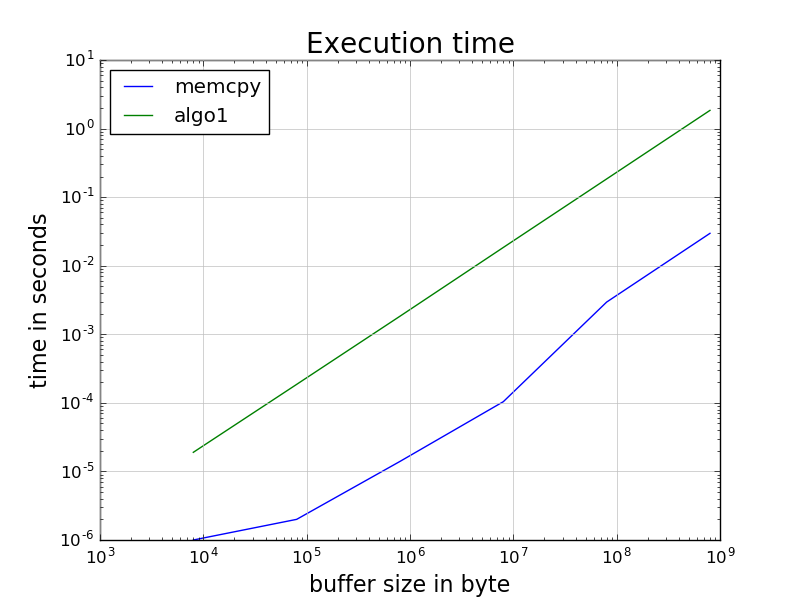
\includegraphics[width=\textwidth,height=0.8\textheight,keepaspectratio]{time.png}
	\end{center}
\end{frame}

\begin{frame}
	\frametitle{Upcoming}

	\begin{itemize}
		\item Implementation of first custom algorithms decompression
		\item Minor project structure and interface changes
		\item Implementation of second custom algorithm
		\item Implementation of algorithms for gzip, bzip2, etc...
		\item Thorough benchmarking
	\end{itemize}

\end{frame}

\end{document}
